\chapter{RESULTADOS}
\label{cap:resultados}

Os resultados obtidos com a presente etapa da pesquisa são de enorme relevância para a futura implementação do projeto, pois determinados aspectos observados, modificaram a decisão a ser tomada quanto a ferramenta que será posteriormente incorporada ao projeto vigente.

A principal ferramenta candidata quanto a incorporação até o momento era CoreNLP, processador de língua natural de Stanford University, uma vez em que tal ferramenta possui uma completa e robusta estrutura para construção das árvores sintáticas bem como quanto a geração de informações necessárias para o sistema a ser trabalhado. Ao detalhar-se o código e a estrutura do CoreNLP, denotou-se que seria necessário a adição e construção de um módulo independente para o idioma português, seguindo a estruturação dos módulos de Árabe, Espanhol, Chinês, Alemão e Francês.

Conforme as execuções, a ferramenta necessita de um corpus textual em um dos determinados idiomas previamente conhecidos pelo CoreNLP e parâmetros para a definição do idioma e métodos de analises a serem utilizados.

\begin{figure}[H]
\centering
\caption{Executando CoreNLP sobre um corpus textual} %legenda
\begin{Verbatim}[fontsize=\small]
$ echo "the quick brown fox jumped over the lazy dog" > input.txt
$ java -mx3g edu.stanford.nlp.pipeline.StanfordCoreNLP -outputFormat json -file input.txt
\end{Verbatim} 
{\small Fonte: Teste executado.} %Fonte da imagem
\label{fig:exemploconfig} %rotulo para refencia
\end{figure}

\begin{figure}[H]
\centering
\caption{Saída CoreNLP sobre um corpus textual} %legenda
\begin{Verbatim}[fontsize=\small]
$ echo "the quick brown fox jumped over the lazy dog" > input.txt
$ java -mx3g edu.stanford.nlp.pipeline.StanfordCoreNLP -outputFormat json -file input.txt
\end{Verbatim} 
{\small Fonte: Teste executado.} %Fonte da imagem
\label{fig:exemploconfig} %rotulo para refencia
\end{figure}

Ao decorrer do estudo sobre a arquitetura da ferramenta, denotou-se que haveria de ser desenvolvido um módulo para o idioma Português brasileiro, no entanto, todos os módulos de todos os idiomas previamente desenvolvidos, usufruem da ferramenta Cogroo, com exceção do idioma Inglês nativo.

Em sua complexa estrutura, a ferramenta conta com um objeto responsável por efetuar o mapeamento do corpus fornecido ao sistema para com os objetivos do usuário, seja aplicar o mecanismo de tagger ou executar uma analise morfossintática sobre cada sentença de entrada.

\begin{figure}[H]
\centering
\caption{Objeto de mapeamento do sistema} %legenda
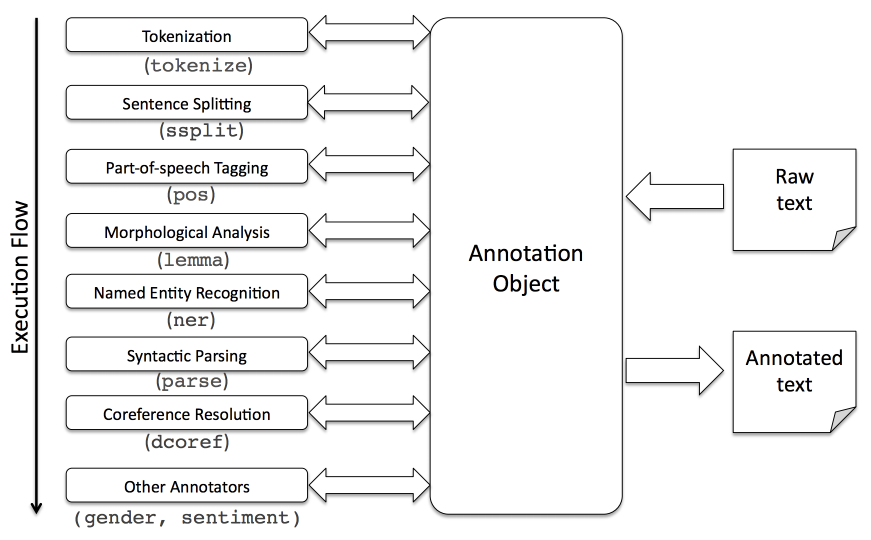
\includegraphics[scale=0.4]{AnnotationPipeline}\\  % o 0.9 indica 90% do tamanho original
{\small Fonte: CoreNLP Community - stanfordnlp.github.io} %Fonte da imagem
\label{fig:exemplo} %rotulo para refencia
\end{figure}

Este mecanismo auxiliaria a integração com o sistema a ser desenvolvido no presente projeto, uma vez em que somente específicas informações e não todas que o CoreNLP oferece seriam necessárias para que fosse possível a extração da informação a partir de um documento de requisitos de entrada.

\begin{figure}[H]
\centering
\caption{Exemplo de invocação dos módulos} %legenda
\begin{lstlisting}
public AnnotationPipeline buildPipeline() {
    AnnotationPipeline pl = new AnnotationPipeline();
    pl.addAnnotator(new TokenizerAnnotator(false));
    pl.addAnnotator(new WordsToSentencesAnnotator(false));
    pl.addAnnotator(new POSTaggerAnnotator(false));
    pl.addAnnotator(new MorphaAnnotator(false));
    pl.addAnnotator(new TimeAnnotator("sutime", props));
    pl.addAnnotator(new PhraseAnnotator(phrasesFile, false));
    return pl;
}
\end{lstlisting} 
{\small Fonte: CoreNLP Community - stanfordnlp.github.io} %Fonte da imagem
\label{fig:exemplocodigo1} %rotulo para refencia
\end{figure}


Segundo os parâmetros passados ou em uma possível integração com outro sistema, por via de APIs, as propriedades configuradas e os métodos invocados através do objeto mapeador, a ferramenta é capaz de gerar as seguintes saídas:

\begin{figure}[H]
\centering
\caption{Trechos de Discurso} %legenda
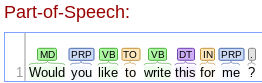
\includegraphics[scale=0.9]{01a}\\  % o 0.9 indica 90% do tamanho original
{\small Fonte: Execução da Ferramenta} %Fonte da imagem
\label{fig:exemplo} %rotulo para refencia
\end{figure}

\begin{figure}[H]
\centering
\caption{Lemas} %legenda
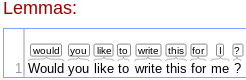
\includegraphics[scale=0.9]{02b}\\  % o 0.9 indica 90% do tamanho original
{\small Fonte: Execução da Ferramenta} %Fonte da imagem
\label{fig:exemplo} %rotulo para refencia
\end{figure}

\begin{figure}[H]
\centering
\caption{Reconhecimento de Entidades} %legenda
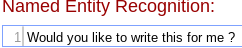
\includegraphics[scale=0.9]{03c}\\  % o 0.9 indica 90% do tamanho original
{\small Fonte: Execução da Ferramenta} %Fonte da imagem
\label{fig:exemplo} %rotulo para refencia
\end{figure}

\begin{figure}[H]
\centering
\caption{Árvore Sintática} %legenda
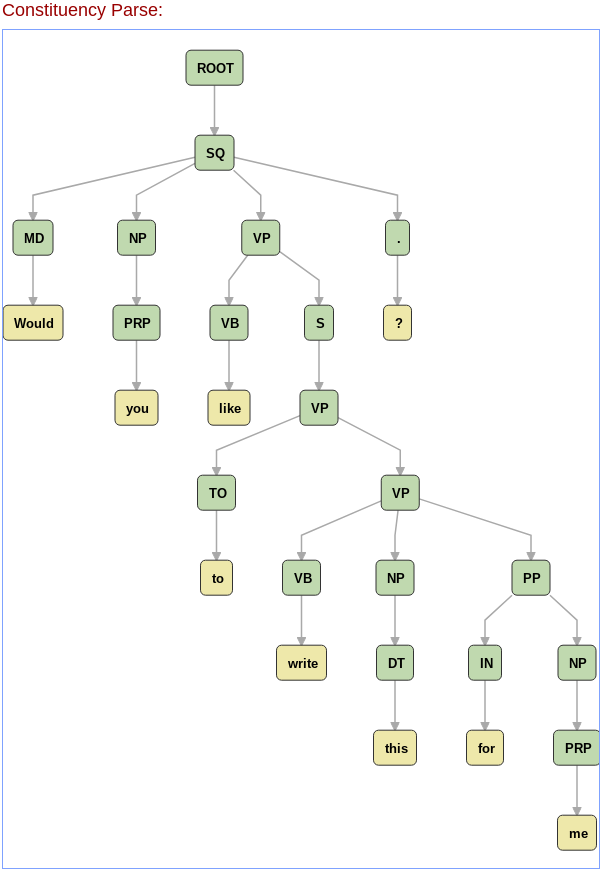
\includegraphics[scale=0.6]{04d}\\  % o 0.9 indica 90% do tamanho original
{\small Fonte: Execução da Ferramenta} %Fonte da imagem
\label{fig:exemplo} %rotulo para refencia
\end{figure}

\begin{figure}[H]
\centering
\caption{Árvore de Dependências} %legenda
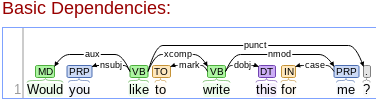
\includegraphics[scale=0.9]{05e}\\  % o 0.9 indica 90% do tamanho original
{\small Fonte: Execução da Ferramenta} %Fonte da imagem
\label{fig:exemplo} %rotulo para refencia
\end{figure}

\begin{figure}[H]
\centering
\caption{Árvore de Dependências} %legenda
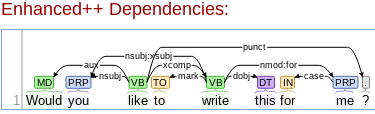
\includegraphics[scale=0.9]{06f}\\  % o 0.9 indica 90% do tamanho original
{\small Fonte: Execução da Ferramenta} %Fonte da imagem
\label{fig:exemplo} %rotulo para refencia
\end{figure}

\begin{figure}[H]
\centering
\caption{IE} %legenda
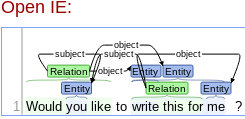
\includegraphics[scale=0.9]{07g}\\  % o 0.9 indica 90% do tamanho original
{\small Fonte: Execução da Ferramenta} %Fonte da imagem
\label{fig:exemplo} %rotulo para refencia
\end{figure}

\begin{figure}[H]
\centering
\caption{Conferência} %legenda
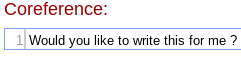
\includegraphics[scale=0.9]{08h}\\  % o 0.9 indica 90% do tamanho original
{\small Fonte: Execução da Ferramenta} %Fonte da imagem
\label{fig:exemplo} %rotulo para refencia
\end{figure}

\begin{figure}[H]
\centering
\caption{Relações KBP} %legenda
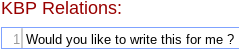
\includegraphics[scale=0.9]{10j}\\  % o 0.9 indica 90% do tamanho original
{\small Fonte: Execução da Ferramenta} %Fonte da imagem
\label{fig:exemplo} %rotulo para refencia
\end{figure}

\begin{figure}[H]
\centering
\caption{Análise de Sentimento} %legenda
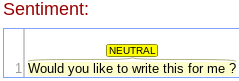
\includegraphics[scale=0.9]{11j}\\  % o 0.9 indica 90% do tamanho original
{\small Fonte: Execução da Ferramenta} %Fonte da imagem
\label{fig:exemplo} %rotulo para refencia
\end{figure}

Outra ferramenta avaliada, Poli-Libras, um sistema de tradução de um corpus textual para Língua Brasileira de Sinais (LIBRAS) intermediado por uma interface gráfica, demonstra-se relevante para o presente projeto, uma vez em que é composta por mecanismos de analise sintática para o idioma português brasileiro, para o qual acarreta grande vantagem em facilitar de desenvolvimento do sistema em questão.

Não existe maneira de se executar o Poli-Libras somente com simples entrada e saída objetivando somente a analise das informações e construções do software como a ferramenta anteriormente discutida, uma vez em que ela foca diretamente na integração com outro sistema através de módulos ou eu seu próprio sistema nativo, com a interface gráfica e outros módulos satélites.

A ferramenta Tagger desenvolvida núcleo NILC, também foi alvo dos estudos na presente etapa do projeto. Caso a opção de ferramenta escolhida fosse o Poli-Libras, haveria necessidade de utilizarmos uma ferramenta do tipo tagger para mapear todo um corpus textual de entrada, no caso, um documento de requisitos, para que fosse possível o parsing e a extração das informações necessárias.

\begin{figure}[H]
\centering
\caption{Exemplo de corpus textual mapeado com o tagger desenvolvido pelo NILC} %legenda
\begin{Verbatim}[fontsize=\small]
._.
Surgiu_VINT ,_, então_ADV ,_, a_ART atualmente_ADV aceita_ADJ 
teoria_N da_PREP+ART biogênese_N ._.
Teoria_N da_PREP+ART abiogênese_N :_: os_ART seres_N vivos_ADJ
originam-se_VBI+PPOA da_PREP+ART matéria_N bruta_ADJ de_PREP 
maneira_N contínua_ADJ ._.
Teoria_N da_PREP+ART biogênese_N :_: os_ART seres_N vivos_ADJ 
originam-se_VBI+PPOA de_PREP outros_ADJ seres_N vivos_ADJ ._.
Von_NP Helmont_NP (_( 1600_NC )_) ,_, o_ART maior_ADJ 
fisiologista_N da_PREP+ART época_N ,_, dá_VTD várias_ADJ 
receitas_N para_PREP a_ART abiogênese_N ._. Uma_ART delas_PREP+PPR
é_VLIG a_ART fórmula_N para_PREP se_PAPASS obter_VTD ratos_N :_: 
"_" enche-se_VBI+PPOA de_PREP trigo_N e_CONJCOORD fermento_N 
um_ART vaso_N ,_, que_PR é_VAUX fechado_VTD com_PREP uma_ART 
camisa_N suja_ADJ ,_, de_PREP preferência_N de_PREP mulher_N ._.
\end{Verbatim} 
{\small Fonte: NILC Website.} %Fonte da imagem
\label{fig:exemploconfig} %rotulo para refencia
\end{figure}

Os conjuntos de tags definidos por padrões internacionais de tagset possibilitam a integração entre a ferramenta de tagger e a ferramenta de processamento de língua natural. Caso a opção escolhida fosse a ferramenta CoreNLP, não haveria necessidade do uso de um tag, haja visto que existem módulos em sua robusta construção, que promovem o mapeamento por meio das tags de um corpus textual de entrada.

Concluindo a presente etapa de pesquisa, analisou-se a ferramenta Cogroo, o corretor gramatical livre e open source da suíte de aplicativos Libre Office. Esta ferramenta destacou-se por estar presente em todas as demais ferramentas supracitadas, exceto Poli-Libras e Nilc Tagger, atraindo o foco para ser a atual e mais provável candidata a incorporação ao sistema. Uma ferramenta robusta, com elevada taxa de acerto na classificação gramatical, possui API de integração com outros sistemas, irá facilitar amplamente o desenvolvimento do projeto em questão.

Cogroo é capaz de prover algumas informações de saída quando recebe um corpus textual como entrada, onde a estrutura resultante mais importante e necessária é a árvore sintática, de onde pode-se extrair os dados relevantes para classificação das estruturas gramaticais presentes no corpus e assim possibilitar a averiguação de estruturas conhecidas como casos de teste, entidades do sistema, dentre outros.

\begin{quadro}[H]
  \begin{center}
    \caption{Exemplo de execução da ferramenta sobre a sentença: "O futuro está em processamento de línguas naturais."} 
    \label{tab:exemplo}
    \vspace{0.1cm}
    \footnotesize
    \begin{tabular}{|c|c|c|c|c|c|c|}
      \hline
      N# & Elemento & Lemas & Classe & Flexão & Sintagma & Função \\
      \hline
      \hline
      1 & O & o & artigo & masculino, singular & nominal & sujeito\\
      2 & futuro & futuro & substantivo & masculino, singular & nominal & sujeito\\
      3 & está & estar & verbo infinitivo & presente, terceira pessoa, singular, indicativo & verbal & predicado\\
      4 & em & em & preposição & - & preposicional & complemento adverbial\\
      5 & processamento & processamento, processar & substantivo & masculino, singular & nominal & complemento adverbial\\
      6 & de & de & preposição & - & preposicional & complemento adverbial\\
      7 & línguas & língua & substantivo & feminino, plural & nominal & complemento adverbial\\
      8 & naturais & natural & adjetivo & feminino, plural & nominal & complemento adverbial\\
      \hline 
    \end{tabular}
  \end{center}
  \centering {\small Fonte: Saída da execução} %Fonte do quadro
\end{quadro}

\begin{figure}[H]
\centering
\caption{Árvore sintática gerada pela ferramenta Cogroo} %legenda
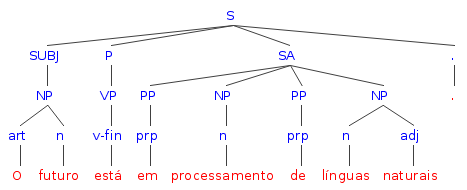
\includegraphics[scale=0.6]{stgraph}\\  % o 0.9 indica 90% do tamanho original
{\small Fonte: Execução da Ferramenta} %Fonte da imagem
\label{fig:exemplo} %rotulo para refencia
\end{figure}

Além do teste e estudo das estruturas e arquiteturas das ferramentas em questão, foi executado uma revisão bibliográfica da literatura objetivando a identificação dos principais métodos para a extração da informação através de documentos textuais, inclusive com trabalhos que especificam documentos de requisitos para empresas de tecnologia da informação. Denotou-se também os principais desafios da aplicação dos métodos de extração de informações com base em problemas já conhecidos do campo de pesquisa em processamento de línguas naturais.

Sabe-se que os principais problemas no tratamento de PLN para o presente projeto enquadra-se em ambiguidade de sentenças, omissão de informação por parte do redator do corpus textual e construções gramaticais não suportadas pela ferramenta de PLN a ser utilizada. Para algum desses desafios, certos autores apresentam soluções como verificado na construção da ferramenta UGMAR [REFERENCIA DO ARTIGO] onde o autor propõe soluções para desambiguação de sentenças, reconstrução de certas informações omitidas, claro que com um nível muito restrito de limitação e arquiteturas para o desenvolvimento destes mecanismos.